
\documentclass[a4wide]{report}
% article: formato de artigo científico
% report: relatórios (só com frente)
% book: livro (frente e verso)
% letter: carta

\usepackage[utf8]{inputenc}
\usepackage[T1]{fontenc}
\usepackage[portuguese]{babel}

\usepackage{url}
\usepackage{graphicx}
\usepackage[pdf]{graphviz}

\bibliographystyle{acm}
\usepackage{ulem} %usado para sublinhar palavras

\usepackage{hyperref}
\usepackage{xcolor}
\hypersetup{
    colorlinks=true,
    urlcolor=blue,
    linkcolor=black,
    citecolor=red
}

% define formato da margem (2 cm)
\usepackage[margin=2cm]{geometry}
\usepackage{titlesec}
% Define o formato da secção
\titleformat{\section}{\LARGE\bfseries}{\thesection}{1em}{}

% listagem de código

\usepackage{listings}
\lstset{language=C}
\lstset{basicstyle=\small,
        captionpos=b,
        float=tp,
        xleftmargin=1.5em,
        xrightmargin=1.5em,
        frameround=ttff,
        frame=single,
       floatplacement=tbp}
\def\lstlistlistingname{Listagens de Código}
\def\lstlistingname{Listagem}


\usepackage{amsmath}

% ---  Página de rosto  --- 
\title{Trabalho Prático \\ 
Laboratórios de Informática }
\author{Docente: Óscar Rafael da Silva Ferreira Ribeiro \\
Escola Superior de Tecnologia \\
Licenciatura em Engenharia de Sistemas Informáticos \\
\\
\\
Realizado por: \\
Pedro Ribeiro nº27960 \\
Ricardo Fernandes nº27961 \\
Carolina Branco nº27983\\}
\date{ \today } % {December 2022}

\begin{document}
\maketitle

\begin{abstract} % resumo
\Large
No âmbito da unidade curricular de Laboratórios de Informática, desenvolvemos um trabalho prático em grupo, abordando o mesmo problema da unidade curricular de Programação Imperativa. Utilizamos uma máquina virtual com "Oracle VM VirtualBox" e "Ubuntu" para criar um programa que atende aos critérios do professor. O objetivo inclui a formulação de um programa com sintaxe clara, manipulação de argumentos e opções, criação de um MakeFile, relatório em LaTeX, documentação com Doxygen, e um repositório no GitHub. O relatório detalha cada etapa do projeto, visando a compreensão dos conceitos lecionados. Buscamos aprimorar habilidades em desenvolvimento de código, manipulação de argumentos, documentação, uso do GitHub, LaTeX e Git, além de trabalhar em equipa. O objetivo geral é diversificar conhecimentos e evitar a passividade na aprendizagem. O projeto visa também melhorar as habilidades de trabalho em grupo, reconhecendo a importância da colaboração para o futuro.

\end{abstract}

% ÍNDICES do documento
% índice global:
\tableofcontents
% figuras
\listoffigures
% tabelas
\listoftables
% listagens de código
\lstlistoflistings


\chapter{Introdução}
%\section{Introdução}
\Large
No âmbito da unidade curricular de Laboratórios de Informática, realizámos como trabalho prático de final de semestre, a produção de um trabalho de grupo. A realização do presente trabalho de grupo tem como problema o mesmo fornecido pelo trabalho prático final da unidade curricular Programação Imperativa. O presente trabalho prático consiste na elaboração de um código, onde serão aplicados os conceitos que foram abordados ao longo do semestre letivo. Para a realização do trabalho foi usada uma máquina virtual, possibilitada pelo uso das aplicações “Oracle VM VirtualBox” e “Ubuntu” Este trabalho objetiva formulação de um programa capaz de atender aos critérios fornecidos pelo professor de Programação Imperativa, além disso objetiva também a associação ao comando uma sintaxe de utilização, possibilitando a passagem dos ficheiros de entrada como argumentos do programa. Além disso possibilita também a entrada de opções. Com este trabalho é pretendida a realização de um ficheiro MakeFile, da formulação de um relatório com a plataforma “LaTex”, o desenvolvimento da documentação do código com a plataforma “Doxygen” e a criação de um repositório no “GitHub”. Além disso para o presente trabalho prático foi nos requerida a realização de um relatório, em que explicamos cada etapa que foi necessária que foi necessária para a realização do mesmo, visando a envolvência e a explicitação dos conceitos que foram lecionados em contexto de sala de aula. Por fim, fomos propostos à realização de apresentações orais, onde pretendemos ter a oportunidade de mostrar o que foi aprendido.

Com a realização do presente trabalho prático, temos como objetivo praticar um conjunto de aptidões para o desenvolvimento em grupo de um projeto de média dimensão usando o paradigma imperativo. Com este trabalho pretendemos desenvolver, aptidões de formulação de código e de lógico da programação. Objetivamos o aprimoramento nas aptidões quanto ao domínio da entrada de argumentos num código, conseguindo a manipulação das mesmas. Além disso pretendemos aprender e consolidar conceitos já abordados pelo professor acerca da documentação do código, bem como compreender e valorizar a sua importância na realização de um bom programa. Por estes motivos pretendemos verificar a pertinência do uso de “Doxygen”. Temos também a intenção de adquirir conhecimentos no “GitHub” e no “Git”, considerámos ambos de extrema importância por entendermos esta, como sendo uma excelente ferramenta colaborativa de trabalho, que permite a elaboração de projetos em grupo e de divulgação de trabalho, daí termos considerado o desenvolvimento do projeto com envolvência nesta plataforma extremamente coerente. Pretendemos que o uso de “LaTex”, tenha também uma influência positiva no nosso desempenho, pois considerámos que seria produtivo e vantajoso a aplicação de novas plataformas ao trabalho de modo a diversificar os conhecimentos. É pretendido também a aquisição de aptidões de desenvolvimento de um ficheiro “README.md” de qualidade, bem como o entendimento da sua importância no desenvolvimento de um projeto. Como objetivo geral, com o trabalhar das diferentes plataformas referidas, pretendemos o desenvolvimento de conhecimento diversificado, permitindo-nos a nós mesmos explorar novos conhecimentos, impedindo a passividade na aprendizagem.

Por fim, e não relacionado diretamente com a unidade curricular pretendemos com este trabalho aprimorar as nossas capacidades de trabalho em grupo, ao perceber que cada pessoa tem o seu método de trabalho e aprendendo retirar o melhor de cada um elaborando o melhor projeto possível. Considerámos esta capacidade relevante pois reconhecemos como sendo de extrema importância para o nosso futuro a capacidade de exercer uma função em conjunto.

\newpage
\chapter{Estrutura do Código}
%\section{Estrutura do Código}

\section{Criação dos Ficheiros .c e .h}
%\section{Criação dos ficheiros .c e .h}
\Large
	Para a realização do projeto usámos uma máquina virtual, inicialmente para o início do nosso projeto tivemos que entrar num repositório no GitHub previamente criado pelo professor. Para fazermos a importação do repositório para a máquina usámos o comando “git pull”. Após o uso deste comando tínhamos assim a pasta do repositório na nossa máquina. Após estes passos, procedemos a criação dos diferentes ficheiros do programa criado no projeto, através do comando “nano” (ex: nano Dados.h).
\begin{figure}[hbt]
    \centering
    
\includegraphics[width=0.40\textwidth]{criacaoficheiros.png}
    \caption{\textbf{\textit{Ficheiros .h e .c criados.}}\label{fig:imagem}}
\end{figure}
	Depois da criação dos ficheiros acima apresentados, com a orientação do professor, após termos experienciado o “vim” como auxiliar de edição de ficheiros, experimentamos a instalação do “vscode”, facilmente percebemos a praticidade do mesmo, portanto foi, o editor usado por todos os elementos do trabalho. 

	Como requerido pelo professor da presente unidade curricular, usamos para este projeto o mesmo enunciado que o trabalho prático final da unidade curricular de Programação Imperativa, então inicialmente copiámos o código do projeto de programação Imperativa e colámos no presente projeto. 

\section{Criação das Funções}
\Large
%\section{Criação das Funções}

	Após isto, devido a necessidade de pôr como argumentos ficheiros de entrada para o programa, reparámos que o código copiado, necessitava de alterações. Inicialmente reparámos que deveríamos acrescentar funções de leitura dos ficheiros que posteriormente seriam passados por argumentos. Daí procedemos à criação das seguintes funções. 

\newpage
\subsection{Funções LeDados}
\Large

Função de ler os dados dos pacientes, de ler os dados das dietas e de ler dados dos planos nutricionais a partir de ficheiros, respetivamente:

\begin{lstlisting}[language=C, caption={Funções de ler dados}, label={lst:exemplo-c}]
bool LeDadosPacientes(char separador, char fileName[], Paciente *dados,
  int maximoplanos) {

    FILE* fp;
    fp = fopen(fileName, "r");
    if (fp == NULL) {
        return false;
    }
    if (separador == ';') {
        for (int i = 0; i < maximoplanos; i++) {
            fscanf(fp, "%d;%99[^;];%d", &dados[i].numpaciente, dados[i].nome,
            &dados[i].telefone);
            //Para verifcar o que foi lido:
            //printf("dados lidos :%d;%s;%d\n", dados[i].numpaciente, dados[i].nome,
            dados[i].telefone);
        }
    }
    if (separador == '\t') {
        for (int i = 0; i < maximoplanos; i++) {
            fscanf(fp, "%d\t%99[^\t]\t%d", &dados[i].numpaciente, dados[i].nome,
            &dados[i].telefone);
            //Para verifcar o que foi lido:
            //printf("lidos : %d\t%s\t%d\n", dados[i].numpaciente, dados[i].nome,
            dados[i].telefone);
        }
    }
    fclose(fp);
    return true;
}


bool LeDadosDieta(char separador, char fileName[], Dieta *dietas, int maximodietas) {
    FILE * fp;
    fp = fopen (fileName,"r");
    if (fp == NULL) {
    return false; // Retorna false se o apontador do ficheiro for nulo
    }
    if (separador == ';') {
        for (int i = 0; i < maximodietas; i++) {
            fscanf(fp, "%d;%99[^;];%99[^;];%d;%99[^;];%d", &dietas[i].numpaciente,
            dietas[i].datainicio, dietas[i].datafim, &dietas[i].tp,
dietas[i].alimento, &dietas[i].calorias);
            //Para verifcar o que foi lido:
            //printf("%d;%s;%s;%d;%s;%d\n", dietas[i].numpaciente,
            dietas[i].datainicio, dietas[i].datafim, dietas[i].tp,
dietas[i].alimento, dietas[i].calorias);

        }
    }
    if (separador == '\t') {
        for (int i = 0; i < maximodietas; i++) {
            fscanf(fp, "%d\t%99[^\t]\t%99[^\t]\t%d\t%99[^\t]\t%d",
&dietas[i].numpaciente, dietas[i].
            datainicio, dietas[i].datafim, &dietas[i].tp,
dietas[i].alimento, &dietas[i].calorias);
            //Para verifcar o que foi lido:
            //printf("%d\t%s\t%s\t%d\t%s\t%d\n", dietas[i].numpaciente,
            dietas[i].datainicio, dietas[i].datafim, dietas[i].tp,
dietas[i].alimento, dietas[i].calorias);
        }
    }
    fclose(fp);
    return true;
}

bool LeDadosPlanoNutri(char separador, char fileName[], PlanoNutri *nutri,
int maximodados) {
    FILE * fp;
    fp = fopen(fileName,"r");
    if (fp == NULL) {
        return false; // Retorna um dado vazio se o apontador do ficheiro for nulo
    }

    if (separador == ';') {
        for (int i = 0; i < maximodados; i++) {
            fscanf(fp, "%d;%99[^;];%99[^;];%d;%d;%d", &nutri[i].numpaciente,
            nutri[i].datainicio, nutri[i].datafim, &nutri[i].tp,
&nutri[i].caloriasMin, &nutri[i].caloriasMax);
            //Para verifcar o que foi lido:
            //printf("%d;%s;%s;%d;%d;%d\n", nutri[i].numpaciente,
            nutri[i].datainicio, nutri[i].datafim, nutri[i].tp,
nutri[i].caloriasMin, nutri[i].caloriasMax);
        }
    }

    if (separador == '\t') {
        for (int i = 0; i < maximodados; i++) {
            fscanf(fp, "%d\t%99[^\t]\t%99[^\t]\t%d\t%d\t%d", &nutri[i].numpaciente,
            nutri[i].datainicio, nutri[i].datafim, &nutri[i].tp,
&nutri[i].caloriasMin, &nutri[i].caloriasMax);
            //Para verifcar o que foi lido:
            //printf("%d\t%s\t%s\t%d\t%d\t%d\n", nutri[i].numpaciente,
            nutri[i].datainicio, nutri[i].datafim, nutri[i].tp,
nutri[i].caloriasMin, nutri[i].caloriasMax);
        }
    }
    fclose(fp);
    return true;
}

}
\end{lstlisting}
	

A estrutura de todas as funções é semelhante. Inicialmente é declarado como apontador de um ficheiro o “fp”, tal é feito através do comando “FILE * fp”. A linha seguinte do código “fp = fopen (fileName,”r”)” associamos o apontador anteriormente declarado, a abrir o ficheiro cujo o nome é dado por parâmetro à função, para leitura (devido ao uso do caracter “r”). 

	Como proposto pelo professor, o utilizador teria de ter a opção de manipulação de ficheiros csv separados por “;” e separados por tab, então, após estas duas linhas de código, utilizamos if’s para descobrir qual o separador de ficheiro que o utilizador usou nos seus ficheiros. Em cada um dos if’s quer seja o separador “;” ou tab, foi posto um ciclo for de modo a ser possível a iteração pelas linhas dos ficheiros. 

\newpage
Através do fscanf foi possível guardar os dados dos pacientes, das dietas e dos planos nas seguintes structs, respetivamente:  

\begin{figure}[hbt]
    \centering
    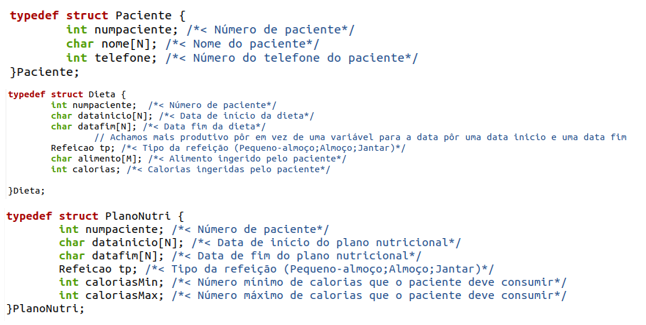
\includegraphics[width=0.80\textwidth]{structs.png}
    \caption{\textbf{\textit{Structs.}}\label{fig:imagem}}
\end{figure}

Por fim, acabámos a edição do ficheiro através da linha de comando “fclose(fp);” e retornamos o valor “true” da função. 

\subsection{Função MostraAjuda}
\Large
Além destas funções como pedido também, fizemos uma função de mostrar ajuda: 

\begin{figure}[hbt]
    \centering
    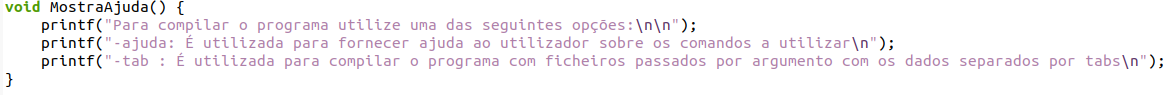
\includegraphics[width=0.90\textwidth]{mostraajuda.png}
    \caption{\textbf{\textit{Função MostraAjuda.}}\label{fig:imagem}}
\end{figure}

NOTA: Após uma sessão de atendimento com o professor, foi-nos dito que poderíamos não utilizar a opção ”-bin”, pois não foram manipulados quaisquer ficheiros binário no trabalho prático final da unidade curricular de Programação Imperativa

\section{Manipulação do main.c}
%\section{Manipulação do main.c}

\subsection{Inserção de Parâmetros na função main}

\Large
Após a realização das funções acima indicadas, fizemos o código necessário no main. O código desenvolvido pode ser divido em várias partes: 

Inicialmente pusemos como argumentos do main o argc e o agrv: 

\begin{figure}[hbt]
    \centering
    
\includegraphics[width=0.40\textwidth]{main.png}
    \caption{\textbf{\textit{Parâmetros da função main.}}\label{fig:imagem}}
\end{figure}


\subsection{Declaração de variáveis}

\Large
Após isto criámos a variável do separador, que por omissão está definida como sendo “;”, criámos também 3 variáveis diferentes também do tipo char, é nestas variáveis que serão guardados os nomes dos ficheiros passados por argumentos. Foi-nos proposto pelo professor para em argumentos por os ficheiros na seguinte ordem: pacientes, dietas e planos nutricionais. Caso não fosse posto o ficheiro relacionado aos planos nutricionais teriam de ser adicionados por standard input. Com isto tivemos a necessidade de fazer algo que distingue se foram colocados os 3 ficheiros ou apenas 2 deles. Para isso criámos a variável main que assume valor 1 se forem inseridos os 3 ficheiros e 0 em caso contrário. Por fim criámos 3 arrays das diferentes structs dos diferentes dados, onde serão guardados os dados inseridos por argumento e/ou por stdin.

\begin{figure}[hbt]
    \centering
    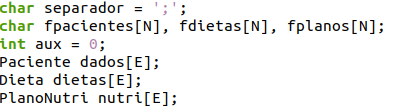
\includegraphics[width=0.40\textwidth]{variaveis.png}
    \caption{\textbf{\textit{Variáveis.}}\label{fig:imagem}}
\end{figure}

\subsection{Análise de argumentos de linha de comando e linha de entrada}

\Large
Após a declaração das variáveis acima analisadas, fizemos a porção do código destinada à leitura dos argumentos a partir dos dados fornecidos por argumentos. 

\begin{lstlisting}[language=C, caption={Código para análise argumentos}, label={lst:exemplo-c}]
if (argc < 3 && strcmp(argv[1], "-ajuda")!=0){
        printf ("Número insuficiente de argumentos");
        return 0;
    } 
    if (strcmp(argv[1], "-ajuda") == 0) {
        MostraAjuda();
        return 0;
    }
    if (strcmp(argv[1], "-tab") == 0) {
        if(argc < 4){
            printf ("Número insuficiente de argumentos\n");
            return 0;
        }else{
            separador = '\t';
            strcpy(fpacientes, argv[2]);
            strcpy(fdietas, argv[3]);
            if (argc == 5) {
                strcpy (fplanos, argv[4]);
                aux = 1;
            }
        }
    }
    else {
        if(argc < 3){
            printf ("Número insuficiente de argumentos\n");
            return 0;
        }else{
            strcpy(fpacientes, argv[1]);
            strcpy(fdietas, argv[2]);
            if (argc == 4) {
                strcpy (fplanos, argv[3]);
                aux = 1;
            }
        }
    }
\end{lstlisting}

O primeiro “if”, é destinado a encerrar o programa caso não existam argumentos suficientes e não seja pedida a ajuda. Isto pois se o utilizador digitar menos de 3 argumentos é impossível, para o código feito, ter os dados suficientes para as funções, isto a menos que o argv[1] seja a opção “-ajuda”. Com isto através do printf o utilizador é notificado da falta de argumentos e o programa para de correr. 

No “if” seguinte caso o utilizador utilize a opção “-ajuda” é mostrada a função a esse fim destinada e o programa par também de correr 

O “if” seguinte é feito para caso o utilizador queira manipular ficheiros com os valores divididos por um tab, isto porque para o utilizador usar ficheiros deste tipo tem que por o argv[1] como -tab. Neste caso, se o argc for menor que 4 não foram colocados argumentos suficientes por isso o utilizador é notificado e o programa encerra. Caso o argc não seja < 4, então a variável anteriormente declarada, separador, toma o valor de tab, o fpacientes toma o valor do nome do ficheiro dos dados dos pacientes, o fdietas toma o valor do nome do ficheiro dos dados dos pacientes e caso o argc seja igual a 5 o fplanos toma o valor do nome do ficheiro dos planos nutricionais, além disso a variável aux toma o valor de 1, avisando posteriormente a não necessidade de passar dados por stdin. 

O else associado ao if abordado, refere-se a quando o utilizador não coloca nenhuma opção, sendo por esse motivo o separador, por omissão, igual a “;”. Neste caso, se o argc for menor que 3 não foram colocados argumentos suficientes por isso o utilizador é notificado e o programa encerra. Caso o argc não seja < 3, fpacientes toma o valor do nome do ficheiro dos dados dos pacientes, o fdietas toma o valor do nome do ficheiro dos dados dos pacientes e caso o argc seja igual a 4 o fplanos toma o valor do nome do ficheiro dos planos nutricionais, além disso a variável aux toma o valor de 1, avisando posteriormente a não necessidade de passar dados por stdin. 

Após isto, caso a variável aux seja ainda igual a 0, o programa iria corresponder à condição de um if destinado à possibilitação de passagem dados por stdin, que será abordado posteriormente. 

\subsection{Análise de dados fornecidos por stdin}

\Large
Como abordado anteriormente, se a variável aux tiver o valor de 0, o programa irá correr as linhas de código presentes dentro do if asseguir: 

\begin{lstlisting}[language=C, caption={Código para análise de dados fornecidos por stdin}, label={lst:exemplo-c}]
    if (aux == 0) {
        char linha[E][1000];
        int i=0;
        while (i < E && fgets(linha[i], 1000, stdin) != NULL) {
            if (linha[i][0] == '\n') {
                printf("Fim da entrada.\n");
                break;
            }
        i++;
        }

        for (int j = 0; j < i; j++) {
            printf("Dados lidos: %s", linha[j]);
        }
        
        FILE *fplanosFILE;

        if (separador == ';') {
            fplanosFILE = fopen("planosstdin.csv", "w");
            strcpy(fplanos,"planosstdin.csv");
        } else if (separador == '\t') {
            fplanosFILE = fopen("tplanosstdin.csv", "w");
            strcpy(fplanos,"tplanosstdin.csv");
        } else {
            printf("Separador não suportado.\n");
            return 1;
        }

        if (fplanosFILE == NULL) {
            perror("Erro ao abrir o ficheiro de planos");
            return 1;
        }

        for (int j = 0; j < i; j++) {
            fputs(linha[j], fplanosFILE);
        }   

        fclose(fplanosFILE);

    }
\end{lstlisting}

Inicialmente fazemos a leitura de entrada, da seguinte forma: 

Com a linha de código “char linha[E][1000];”: declaramos um array bidimensional chamado linha com E linhas e cada linha pode armazenar até 1000 caracteres. Após isso “int i=0;” Inicializa uma variável i com o valor 0 para rastrear o índice das linhas lidas. 

Com o while iniciamos um loop enquanto o índice i é menor que E e a função fgets lê uma linha do stdin (entrada padrão) e armazena na matriz linha[i]. O loop continua enquanto a leitura for bem-sucedida e não atingir o número máximo de linhas E. Dentro desse while temos o “if“, que verifica se a primeira posição da linha lida contém apenas um caractere de nova linha, indicando o fim da entrada. 

Dentro do if, o “printf("Fim da entrada.");” imprime uma mensagem indicando o fim da entrada e depois o “break;”, faz sair do loop. 

O “i++;” incrementa o índice i para a próxima linha. 
Após a leitura dos dados fizemos uma impressão dos mesmos: 

 

Com o ciclo “for (int j = 0; j < i; j++) {“ inicia-se um loop para percorrer as linhas lidas até o índice i. O printf imprime cada linha lida. 
Após isso fazemos a Manipulação de ficheiro: 

 

A linha “FILE *fplanosFILE;” declara um apontador do ficheiro.  

O “if (separador == ';') {“ verifica se a variável separador é igual a “;”. Neste caso, “fplanosFILE = fopen("planosstdin.csv", "w");” abre um ficheiro chamado "planosstdin.csv" para escrita e “strcpy(fplanos, "planosstdin.csv");” copia o nome do ficheiro para a variável fplanos. 

O “} else if {“ verifica se o separador é um tab (\t). Neste caso, “fplanosFILE = fopen("tplanosstdin.csv", "w");” abre um ficheiro chamado "tplanosstdin.csv" para escrita e “strcpy(fplanos, "tplanosstdin.csv");” copia o nome do ficheiro para a variável fplanos. 

O “} else {“ faz com que se o separador não for suportado, o “printf("Separador não suportado");”, imprima uma mensagem de erro e o “return 0;” encerra o programa. 
Escrita no ficheiro: 

 

O “if (fplanosFILE == NULL) {“ verifica se houve erro ao abrir o arquivo e notifica o utilizador através de “perror("Erro ao abrir o ficheiro de planos");” que imprime uma mensagem de erro detalhada e “return 0;” encerra o programa. 

O ciclo “for (int j = 0; j < i; j++) {“ inicia um loop para escrever as linhas no arquivo e “fputs(linha[j], fplanosFILE);” escreve cada linha no ficheiro usando fputs. 
Fechamento do ficheiro: 

 

O “fclose(fplanosFILE);” fecha o arquivo após a escrita. 


\subsection{Leitura e armazenamento dos dados}
\Large

\begin{figure}[hbt]
    \centering
    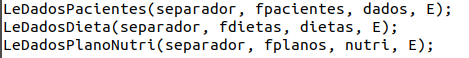
\includegraphics[width=0.55\textwidth]{funcoes.png}
    \caption{\textbf{\textit{Funções de leitura e armazenamento dos dados.}}\label{fig:imagem}}
\end{figure}


Com os valores anteriormente obtidos, já é possível correr as seguintes funções e por isso armazenar os dados necessários e correr o resto do programa 

\section{Desenvolvimento dos ficheiros para uso como argumentos}
\Large
Por fim, procedemos à criação dos diferentes ficheiros, através do comando nano <nome do ficheiro>. 

NOTA: os ficheiros cujo nome se inicia por t são referentes aos ficheiros com separador “tab”, os restantes são com “;”. 

\begin{figure}[hbt]
    \centering
    
\includegraphics[width=0.55\textwidth]{ficheiroscsv.png}
    \caption{\textbf{\textit{Ficheiros para uso como argumentos.}}\label{fig:imagem}}
\end{figure}

\newpage
\chapter{README.md}
\Large
Um ficheiro README.md (Markdown) é um documento de texto formatado usado para fornecer informações sobre um projeto ou repositório. Este tipo de ficheiros é frequentemente encontrado em repositórios de código-fonte, no nosso caso na plataforma GitHub. O README.md serve como uma introdução rápida e guia para utilizadores, desenvolvedores ou colaboradores que exploram o projeto. Utilizando a linguagem de marcação Markdown, o README.md permite uma formatação de texto simples e legível, incluindo cabeçalhos, listas, links e formatação de código.

\section{Estrutura do Ficheiro}
\Large
O ficheiro README.md possui vários cabeçalhos ou campos definidos por cardinais. Quando encontramos apenas um cardinal (por exemplo Trabalho prático) estamos perante um cabeçalho de primeiro nível que se assemelha a um título principal. Se encontrarmos dois cardinais (por exemplo grupo 18) estamos perante um cabeçalho de segundo nível que se assemelha a um subtítulo. Por fim, quando encontramos três cardinais (por exemplo Compilação com make) estamos perante um cabeçalho de terceiro nível e por adiante. 

\newpage
\section{Detalhes de cada cabeçalho}
\Large
Primeiramente temos o cabeçalho de primeiro nível (Trabalho Prático) que é o local de início do ficheiro que apenas possui algumas informações como o nome do curso frequentado e o nome da unidade curricular em questão. 

\begin{figure}[hbt]
    \centering
    \includegraphics[width=0.55\textwidth]{figura1.png}
    \caption{\textbf{\textit{Cabeçalho de primeiro nível.}}\label{fig:imagem}}
\end{figure}

O ficheiro README.md apresenta três cabeçalhos de segundo nível distintos. O primeiro diz respeito ao nome do grupo (grupo 18) e apresenta os detalhes numa tabela sobre os membros do grupo.Exemplo da tabela em questão: 

\begin{table}[h]
\centering
\begin{tabular}{|c|l|}
\hline
\textbf{Número} & \textbf{Nome}          \\ \hline
27960           & Pedro Ribeiro          \\ \hline
27961           & Ricardo Fernandes     \\ \hline
27983           & Carolina Branco       \\ \hline
\end{tabular}
\caption{\textbf{Membros do Grupo 18}\label{tab:grupo18}}
\end{table}


Seguidamente o próximo cabeçalho (Organização) descreve a estrutura e organização do projeto, isto é, possui links que ajudam no acesso a determinadas informações relativas ao projeto. O primeiro link direciona para a documentação gerada pelo Doxygen. Seguidamente, o próximo link direciona para a localização deste mesmo relatório em PDF. Por fim, o último link direciona para o diretório do código-fonte da solução desenvolvida. 

\begin{figure}[hbt]
    \centering
    \includegraphics[width=0.80\textwidth]{figura3.png}
    \caption{\textbf{\textit{Segundo cabeçalho de segundo nível.}}\label{fig:imagem}}
\end{figure}

\newpage
Por fim, o último cabeçalho de segundo nível (Compilação e execução) é composto por três cabeçalhos de terceiro nível, sendo eles “Compilação com make”, “Opções de execução” e “Comandos de execução”. 

No primeiro cabeçalho de terceiro nível (Compilação com make) é explicada a forma como se compila o programa, isto é, acendendo ao terminal e executando o comando “make”. 

\begin{figure}[hbt]
    \centering
    \includegraphics[width=0.55\textwidth]{figura4.png}
    \caption{\textbf{\textit{Primeiro cabeçalho de terceiro nível.}}\label{fig:imagem}}
\end{figure}

Seguidamente, no segundo cabeçalho de terceiro nível (Opções de execução), estão indicadas todas as opções que o Makefile oferece para execução do programa de diferentes maneiras, por exemplo a opção run2f, a opção ajuda, entre outras. 

\begin{figure}[hbt]
    \centering
    \includegraphics[width=0.55\textwidth]{figura5.png}
    \caption{\textbf{\textit{Segundo cabeçalho de terceiro nível.}}\label{fig:imagem}}
\end{figure}

Por último, o último cabeçalho de terceiro nível (Comandos de execução) informa sobre os diversos comandos de execução que podem ser feitos no terminal, por exemplo make run2f, make ajuda, entre outros. 

\begin{figure}[hbt]
    \centering
    \includegraphics[width=0.55\textwidth]{figura6.png}
    \caption{\textbf{\textit{Último cabeçalho de terceiro nível.}}\label{fig:imagem}}
\end{figure}

\newpage
Por fim, o último cabeçalho de terceiro nível (Divisão de tarefas) faz uma pequena descrição sobre a divisão de tarefas para o presente trabalho

\begin{figure}[hbt]
    \centering
    \includegraphics[width=0.55\textwidth]{figura15.png}
    \caption{\textbf{\textit{Último cabeçalho de segundo nível.}}\label{fig:imagem}}
\end{figure}

\newpage
\chapter{Makefile}
\Large
Um Makefile é um ficheiro de configuração usado em projetos de software para automatizar o processo de compilação e execução de tarefas. Este contém regras e diretrizes que especificam como o código-fonte deve ser compilado, quais ficheiros ou dependências estão envolvidos, e como os executáveis compilados devem ser gerados. O Makefile é usado com a ferramenta make, que interpreta as suas instruções e executa as ações correspondentes.

\section{Componentes do Makefile}
\Large
Como componentes principais de um Makefile temos: 

- Regras/Alvos (Targets): Representam as tarefas a serem executadas, como compilar o código, gerar documentação ou executar o programa. 

- Dependências: Na maioria dos casos são objetos, ou seja, ficheiros intermediários gerados durante o processo de compilação do programa, ou até mesmo outras regras. Assim as dependências são ficheiros ou regras necessárias para o funcionamento de uma regra/alvo. 

- Comandos: Instruções específicas a serem executadas para atingir o alvo. Como por exemplo um comando para compilação ou execução de um programa. 

\section{Estrutura do Makefile}
\Large
Primeiramente decidimos definir uma regra padrão “all” que depende do alvo “exec”. Quando se executa o comando make sem especificar qualquer regra, será criado o “exec”.
\\
\begin{figure}[hbt]
    \centering
    \includegraphics[width=0.20\textwidth]{figura7.png}
    \caption{\textbf{\textit{Regra padrão all.}}\label{fig:imagem}}
\end{figure}

\newpage
Por sua vez, definimos a regra “exec” que depende dos objetos main.o , GereDietas.o e GerePacientes.o. Esta regra compila estes objetos num executável chamado "exec" utilizando o comando gcc.

\begin{figure}[hbt]
    \centering
    \includegraphics[width=0.55\textwidth]{figura8.png}
    \caption{\textbf{\textit{Regra exec.}}\label{fig:imagem}}
\end{figure}

Seguidamente definimos os alvos main.o, GereDietas.o e GerePacientes.o, todos eles dependentes dos seus próprios .c’s, isto é, main.c , GereDietas.c e GerePacientes.c respetivamente, e também dos ficheiros cabeçalho, ou seja, Dados.h e Funcoes.h. Estes alvos utilizam o comando gcc para compilar os .c’s em .o’s, ou seja em objetos, neste caso em main.o, GereDietas.o e GerePacientes.o respetivamente

\begin{figure}[hbt]
    \centering
    \includegraphics[width=0.55\textwidth]{figura9.png}
    \caption{\textbf{\textit{Alvos objetos.}}\label{fig:imagem}}
\end{figure}


Por fim definimos as regras que dão origem aos diferentes executáveis:  
\\
\begin{lstlisting}[language=C, caption={Regras que dão origem aos diferentes executácveis}, label={lst:exemplo-c}]

run2f: exec
	./exec Pacientes.csv Dietas.csv

run3f: exec
	./exec Pacientes.csv Dietas.csv PlanosNutri.csv

ajuda: exec
	./exec -ajuda 

tab2f: exec
	./exec -tab tPacientes.csv tDietas.csv

tab3f: exec 
	./exec -tab tPacientes.csv tDietas.csv tPlanosNutri.csv

\end{lstlisting}

\newpage
As regras “run2f” e “run3f” dependem do alvo exec e são destinados a executar o programa com diferentes argumentos. A regra "run2f" executa o programa com dois ficheiros CSV, enquanto "run3f" executa com três ficheiros CSV. 
\\

\begin{figure}[hbt]
    \centering
    \includegraphics[width=0.55\textwidth]{figura10.png}
    \caption{\textbf{\textit{Regras run2f e run3f.}}\label{fig:imagem}}
\end{figure}

A regra ajuda, também depende do alvo exec e é destinada a fornecer ajuda ao utilizador acerca de opções e comandos disponíveis para o programa. 
\\

\begin{figure}[hbt]
    \centering
    \includegraphics[width=0.55\textwidth]{figura11.png}
    \caption{\textbf{\textit{Regra ajuda.}}\label{fig:imagem}}
\end{figure}

As regras “tab2f” e “tab3f” que também dependem do alvo exec, são semelhantes às regras “run2f” e “run3f” mas são destinadas a executar o programa com dados em formato de tabela (separados por tabs).
\\

\begin{figure}[hbt]
    \centering
    \includegraphics[width=0.70\textwidth]{figura12.png}
    \caption{\textbf{\textit{Regras tab2f e tab3f.}}\label{fig:imagem}}
\end{figure}

\newpage
Por último, a regra “clean” que não possui qualquer dependência, remove todos os ficheiros objeto, bem como o executável e ainda os ficheiros criados tanto em caso de ser necessário recorrer a stdin quanto aqueles que foram criados quando são exportados os dados, permitindo assim uma limpeza e organização do diretório do projeto.

\begin{figure}[hbt]
    \centering
    \includegraphics[width=0.80\textwidth]{figura14.png}
    \caption{\textbf{\textit{Regra clean.}}\label{fig:imagem}}
\end{figure}

\chapter{Documetação Doxygen}
\section{Configuração do Doxyfile}
\subsection{1º Passo}
\Large
Para criar um doxyfile é necessário fazer no terminal o comando doxywizard Doxyfile na pasta doc (pasta que vai conter o doxyfile assim como as pastas html e latex) ao fazer este comando vai abrir o Doxygen GUI fronted (Doxyfile).
\begin{figure}[hbt]
    \centering
    
\includegraphics[width=1.00\textwidth]{imagem_1.png}
    \caption{\textbf{\textit{Terminal.}}\label{fig:imagem}}
\end{figure}

\subsection{2º Passo}
\Large
De seguida configuramo-lo devidamente para realizar o que pertendemos. Sendo assim dentro do Wizard Project no “project name” mudamos o nome para Trabalho Prático d-18, no “Source code Directory” colocamos ../src (uma vez que o código realizado se encontra dentro dessa pasta). 
\begin{figure}[hbt]
    \centering
    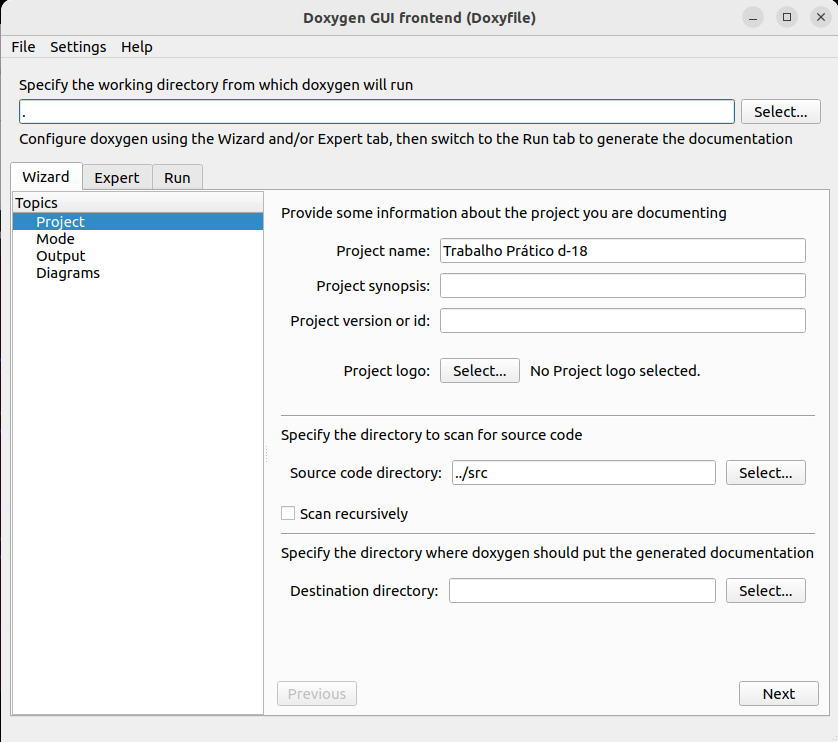
\includegraphics[width=0.40\textwidth]{imagem_2.png}
    \caption{\textbf{\textit{Doxygen GUI}}\label{fig:imagem}}
\end{figure}
\\
\\

\subsection{3º Passo}
\Large
Ainda dentro do wizard mas desta vez no Mode, onde diz “select programming language to optimize the results for:” selecionamos “optimize for C or PHP output”, uma vez que o código realizado se encontra em linguagem C.
\begin{figure}[hbt]
    \centering
    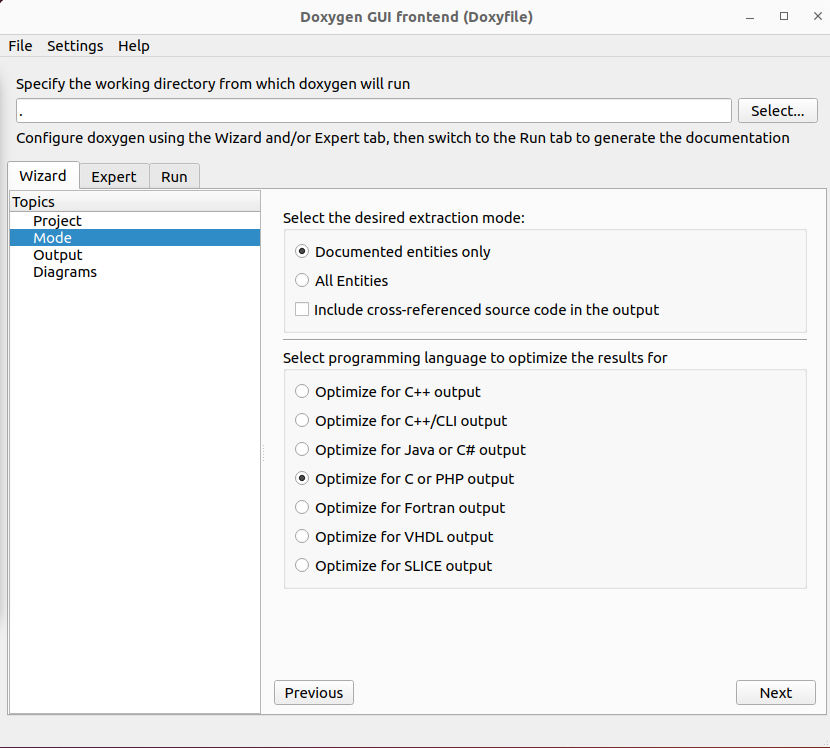
\includegraphics[width=0.40\textwidth]{imagem_3.png}
    \caption{\textbf{\textit{Optimize for C or PHP output}}\label{fig:imagem}}
\end{figure}
\\
\\


\subsection{4º Passo}
\Large
Agora no Expert Build ativamos o "CASE SENSE NAMES", que é uma opção que determina como o Doxygen trata a diferenciação entre maiúsculas e minúsculas nos nomes de classes, funções, variáveis e outros elementos identificadores no código-fonte durante a geração da documentação.
\begin{figure}[hbt]
    \centering
    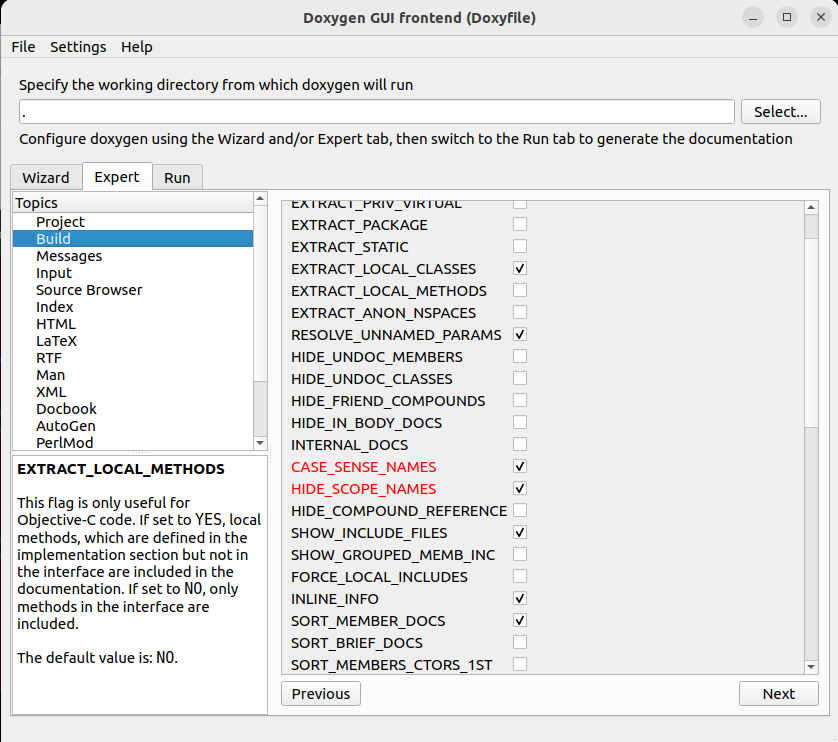
\includegraphics[width=0.40\textwidth]{imagem_4.png}
    \caption{\textbf{\textit{CASE SENSE NAMES}}\label{fig:imagem}}
\end{figure}


\newpage
\subsection{5º Passo}
\Large
Continuando no Build mas agora em Messages ativamos o QUIT que é uma opção utilizada para especificar se o Doxygen deve fechar automaticamente após a geração da documentação ou se deve permanecer aberto.
\begin{figure}[hbt]
    \centering
    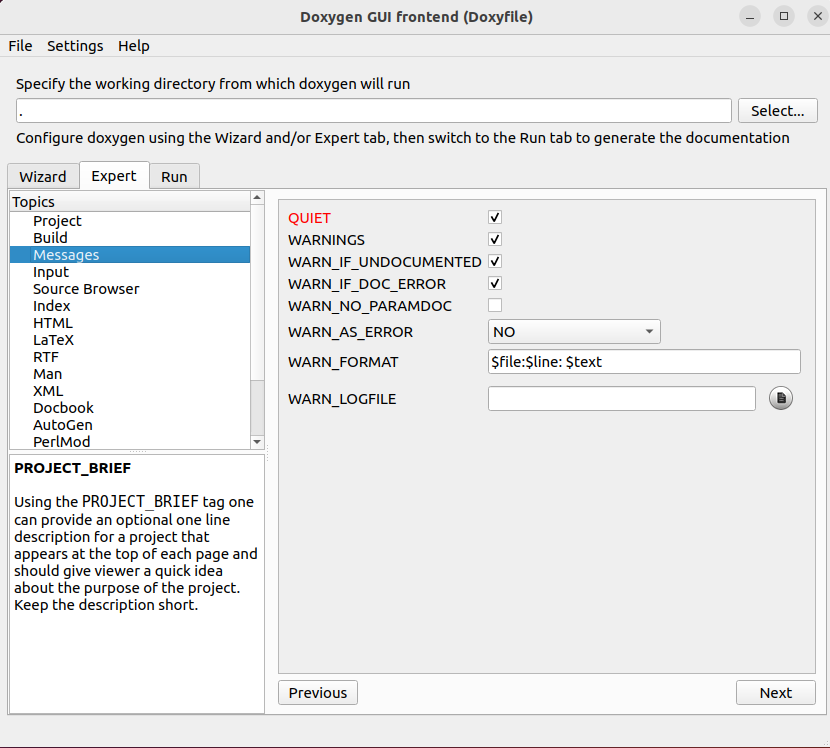
\includegraphics[width=0.40\textwidth]{imagem_5.png}
    \caption{\textbf{\textit{QUIT}}\label{fig:imagem}}
\end{figure}

\subsection{6º Passo}
\Large
De seguida no Expert Input acrescentamos “..” no Input, este serve para especificar os diretórios ou ficheiros que o Doxygen deve analisar para gerar a documentação. Ele indica os locais onde o Doxygen deve procurar os ficheiros de código-fonte e outros ficheiros documentativos.
\begin{figure}[hbt]
    \centering
    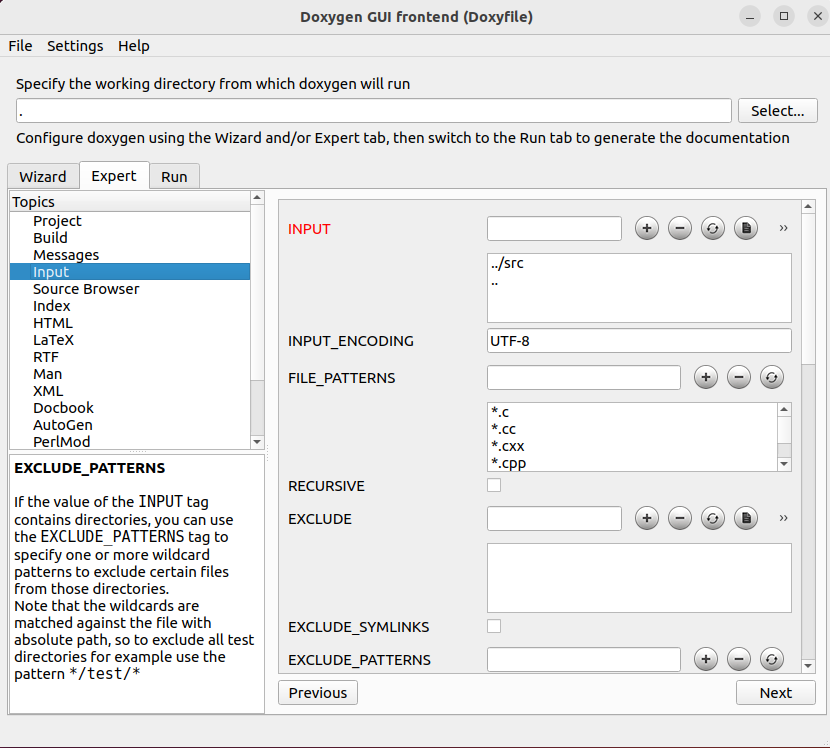
\includegraphics[width=0.40\textwidth]{imagem_6.png}
    \caption{\textbf{\textit{Input}}\label{fig:imagem}}
\end{figure}

\newpage
\subsection{7º Passo}
\Large
Ainda no Expert Input na parte inferior tem o “USE MDFILE AS MAINPAGE” aí colocamos o ficheiro README.md  para ser usado como a página principal (main page) na documentação gerada.  
\begin{figure}[hbt]
    \centering
    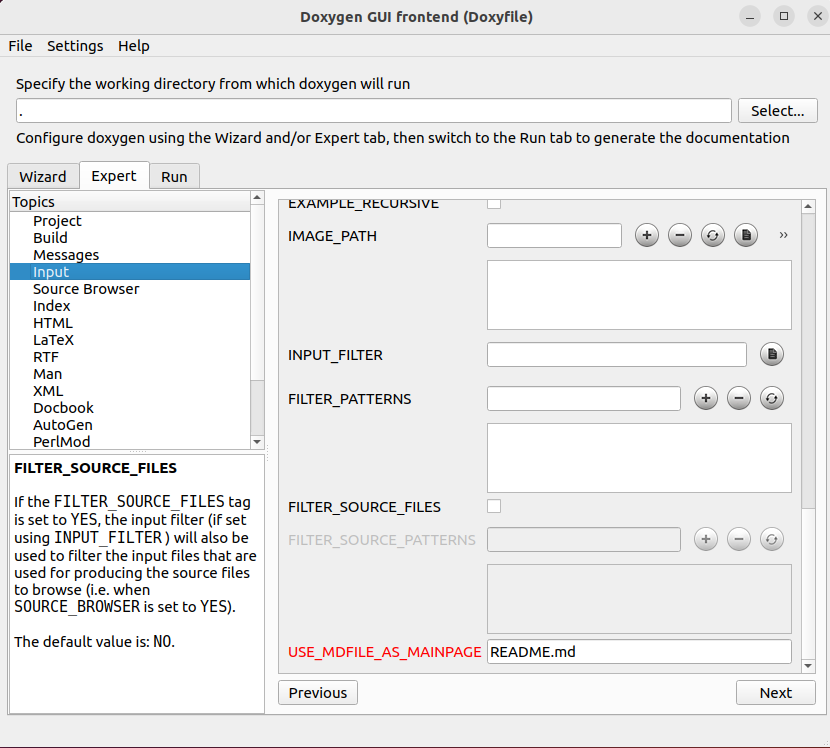
\includegraphics[width=0.40\textwidth]{imagem_7.png}
    \caption{\textbf{\textit{USE MDFILE AS MAINPAGE}}\label{fig:imagem}}
\end{figure}

\subsection{8º Passo}
\Large
Para finalizar a criação do Doxyfile entramos no Run e delecionamos o botão “run doxygen”, ao fazer isto vai gerar automaticamente o Doxyfile assim como as pastas html e latex. 
\begin{figure}[hbt]
    \centering
    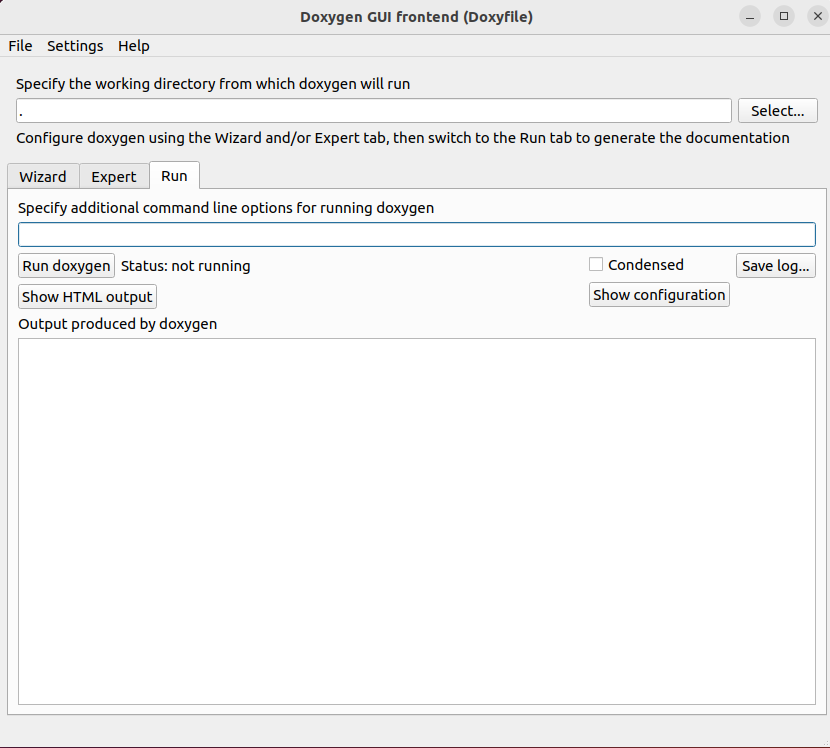
\includegraphics[width=0.40\textwidth]{imagem_8.png}
    \caption{\textbf{\textit{Run doxygen}}\label{fig:imagem}}
\end{figure}



\newpage
\section{Doxygen}
\Large
Para que o código apareça bem estruturado no Doxygen é necessária a sua devida documentação. 

\subsection{Documentação no início de cada ficheiro}
\Large
\begin{figure}[hbt]
    \centering
    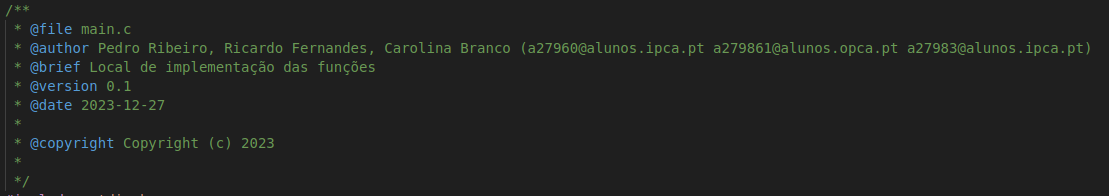
\includegraphics[width=0.70\textwidth]{imagem_121.png}
    \caption{\textbf{\textit{Exemplo da documentação no início de cada}} ficheiro\label{fig:imagem}}
\end{figure}
Fazer esta documentação no início de cada ficheiro faz com que o Doxygen gere um gráfico que vai mostrar a hierarquia entre pastas do sistema de ficheiros.
\begin{figure}[hbt]
    \centering
    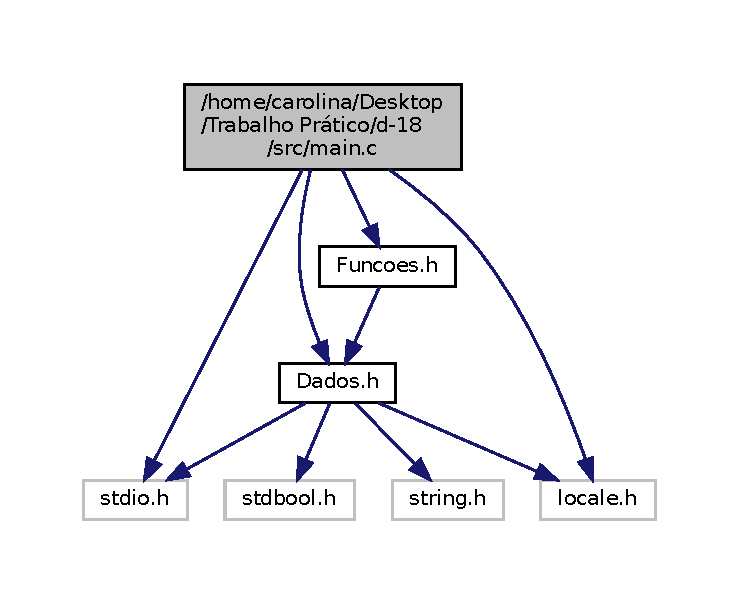
\includegraphics[width=0.40\textwidth]{main_8c__incl.pdf}
    \caption{\textbf{\textit{Gráfico}}\label{fig:image}}
\end{figure}

\subsection{Documentação de Funções}
\Large
Para que o código das funções apareça de devidamente no Doxygen, realizámos a seguinte documentação:
\begin{figure}[hbt]
    \centering
    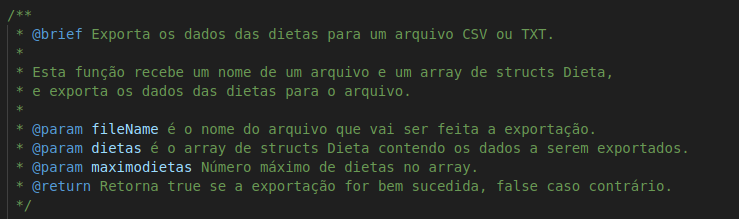
\includegraphics[width=0.70\textwidth]{imagem_13.png}
    \caption{\textbf{\textit{Exemplo de como a documentação deve ser feita}} para cada função\label{fig:imagem}}
\end{figure}

\subsection{Documentação de Structs e Enumerados}
\Large
Para que o código de cada struct/enumereado gere devidamente fizemos a seguinte documentação:
\begin{figure}[hbt]
    \centering
    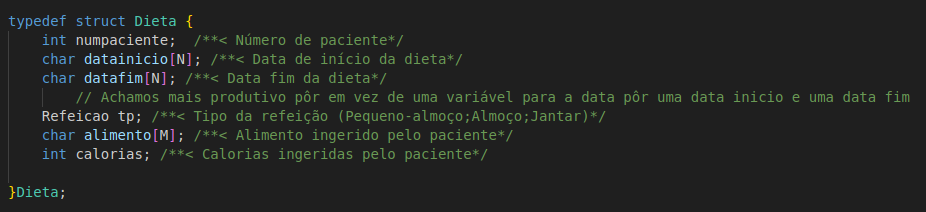
\includegraphics[width=0.70\textwidth]{imagem_14.png}
    \caption{\textbf{\textit{Exemplo de como a documentação deve ser feita para cada struct/enumerado}} \label{fig:imagem}}
\end{figure}








\chapter{Latex}
\section{Ficheiro refman.pdf}
\Large
Para criar o ficheiro refman.pdf utilizamos o ficheiro refman.tex dentro da pasta "latex" gerada pelo Doxygen. Este é um ficheiro  LaTeX que contém o código-fonte LaTeX para a criação da documentação em formato PDF. 
\begin{figure}[hbt]
    \centering
    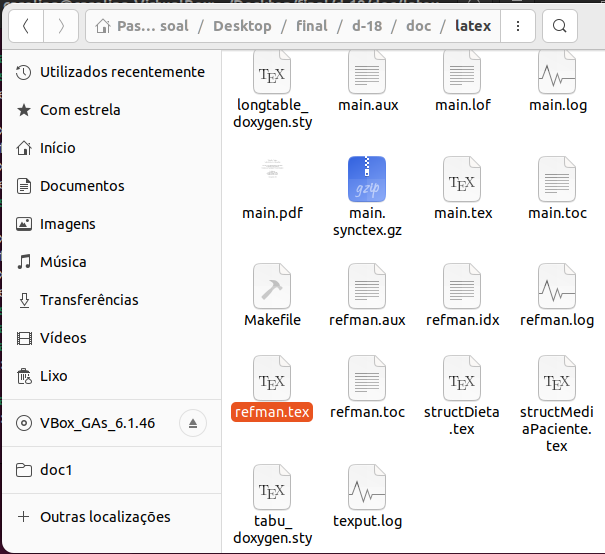
\includegraphics[width=0.40\textwidth]{imagem_15.png}
    \caption{\textbf{\textit{Ficheiro refman.tex}}\label{fig:imagem}}
\end{figure}

Quando utilizamos o Doxygen para gerar a documentação do trabalho, e optamos por ter a documentação em formato LaTeX, com isso o Doxygen cria uma série de ficheiros LaTeX para facilitar a compilação da documentação em diferentes formatos, como PDF. 
O arquivo refman.tex é um desses ficheiros. Ele serve como um ficheiro principal que inclui todos os outros ficheiros LaTeX gerados pelo Doxygen. Esse ficheiro geralmente contém informações sobre a configuração, formatação e comandos LaTeX necessários para compilar a documentação em formato PDF. 
\begin{figure}[hbt]
    \centering
    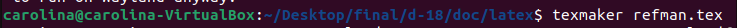
\includegraphics[width=1.00\textwidth]{imagem_16.png}
    \caption{\textbf{\textit{Terminal}} \label{fig:imagem}}
\end{figure}

\newpage
Ao compilar o ficheiro refman.tex usando um compilador LaTeX, como o LaTeX itself ou ferramentas como TeX Live, MikTeX ou Texmaker (ferramenta utilizada neste trabalho) podemos gerar o documento final em formato PDF contendo a documentação completa do nosso trabalho, conforme gerado pelo Doxygen.
\begin{figure}[hbt]
    \centering
    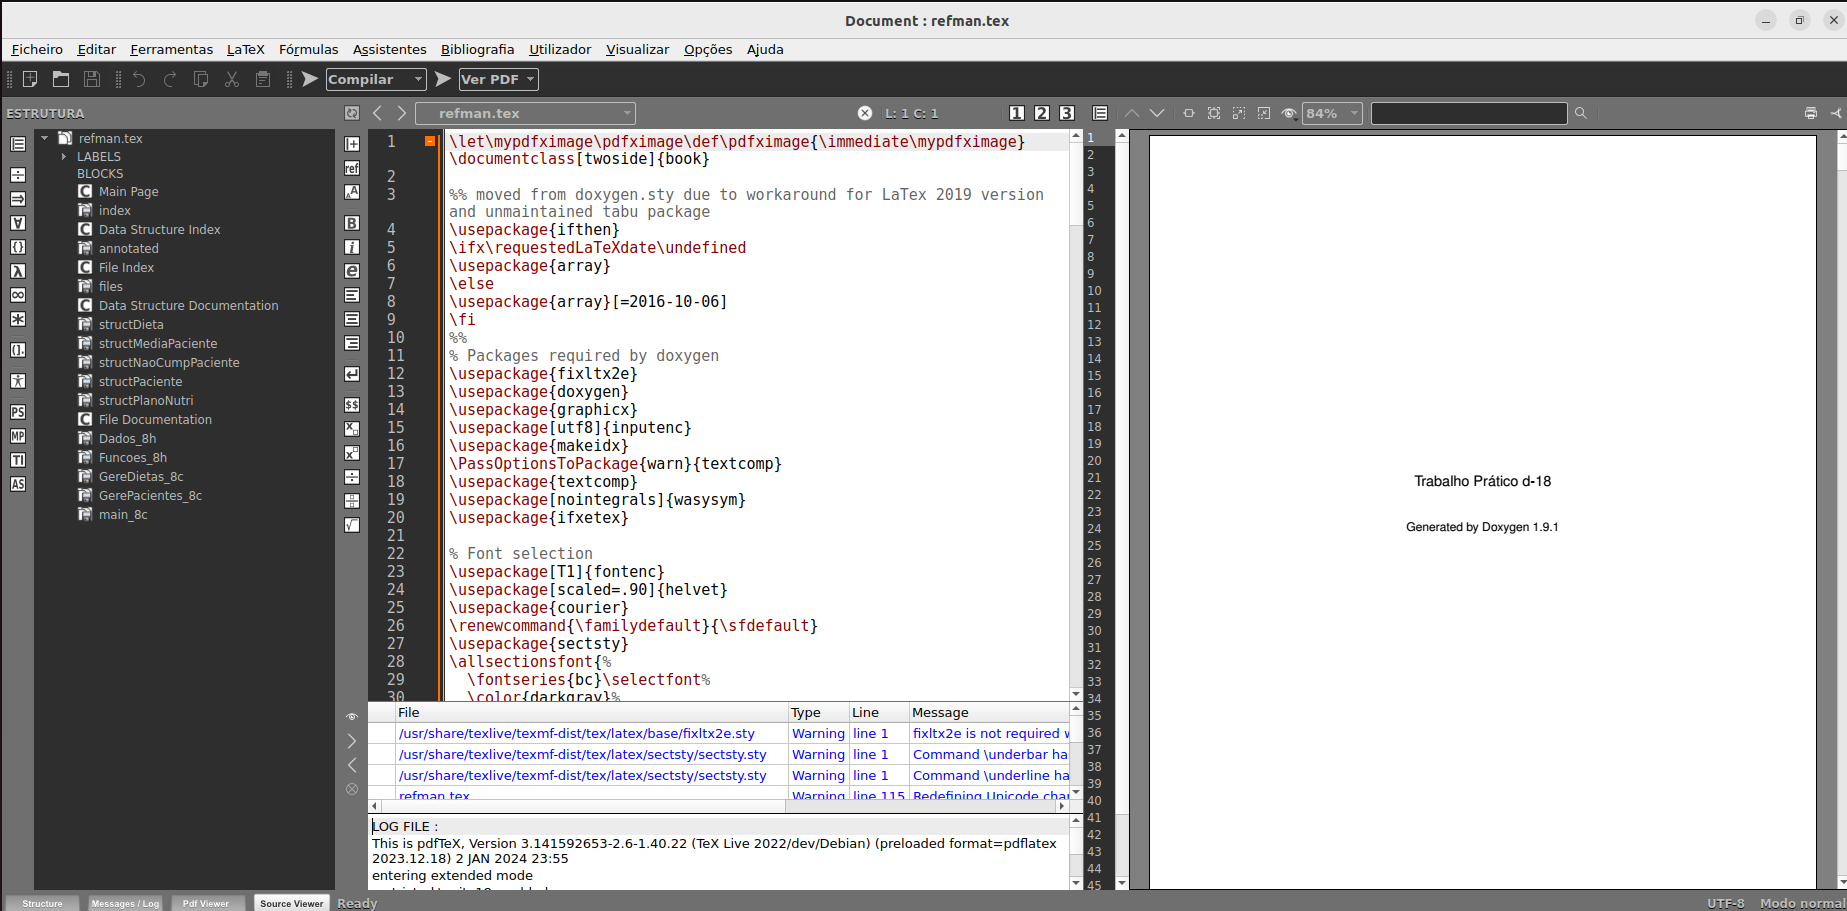
\includegraphics[width=0.70\textwidth]{imagem_17.png}
    \caption{\textbf{\textit{Imagem do texmaker}} \label{fig:imagem}}
\end{figure}

Para abrir o ficheiro refman.tex no Texmaker percisamos de estar na diretório ./d-18/doc/latex (no nosso caso), uma vez que como referido em cima o ficheiro refman.tex encontra-se dentro da pasta latex, e fazer o comando texmaker refman.tex . 
\begin{figure}[hbt]
    \centering
    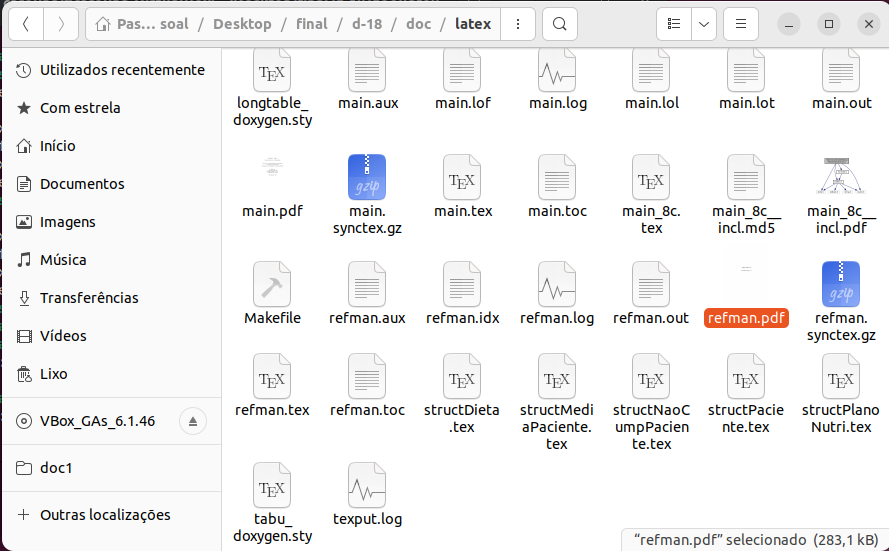
\includegraphics[width=0.40\textwidth]{imagem_18.png}
    \caption{\textbf{\textit{Ficheiro refman.pdf }}\label{fig:imagem}}
\end{figure}



\newpage
\section{Relatório Latex}
\Large
	O relatório LaTex foi gerado a partir da linha de código "texmaker mian.tex". Como pedido pelo professor no presente relatório deve constar os pontos divididos hierarquicamente, por "chapters", "sections" e "subsections", além disso devemos inserir imagens, listagens de código, negrito, itálico e entre outros. Devemos também ter os diferentes indices necessários.
	
\subsection{Como divimos os tópicos hierarquicamente}
\Large
Para dvisão hierarquica dos tópicos usámos com uma barra os comandos "chapter", "section" e "subsection", respetivamente por ordem decrescente hierarquica.

\subsection{Como pusemos o texto em negrito e em itálico}
\Large

\begin{figure}[hbt]
    \centering
    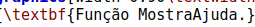
\includegraphics[width=0.40\textwidth]{ima2.png}
    \caption{\textbf{\textit{Comando para texto em negrito}} \label{fig:imagem}}
\end{figure}

\begin{figure}[hbt]
    \centering
    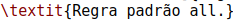
\includegraphics[width=0.40\textwidth]{ima5.png}
    \caption{\textbf{\textit{Comando para texto em itálico}} \label{fig:imagem}}
\end{figure}

\subsection{Como inserimos imagens}
\Large

\begin{figure}[hbt]
    \centering
    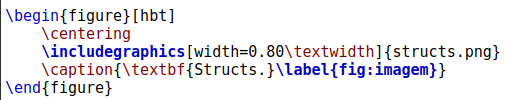
\includegraphics[width=0.40\textwidth]{ima1.png}
    \caption{\textbf{\textit{Comando para inserir imagens}} \label{fig:imagem}}
\end{figure}

\newpage

\subsection{Como inserimos listagem de código}
\Large

\begin{figure}[hbt]
    \centering
    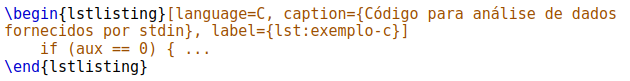
\includegraphics[width=0.45\textwidth]{ima3.png}
    \caption{\textbf{\textit{Comando para inserir listagens de cógigo}} \label{fig:imagem}}
\end{figure}


\subsection{Como inserimos os indíces necessários}
\Large

\begin{figure}[hbt]
    \centering
    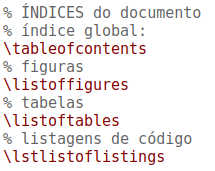
\includegraphics[width=0.30\textwidth]{ima4.png}
    \caption{\textbf{\textit{Comando para inserir índices}} \label{fig:imagem}}
\end{figure}

\chapter{Ficheiro .bib}
\section{Criação e Preenchimento do ficheiro .bib}
\Large
	Para a criação do ficheiro (.bib), ficheiro responsável por armazenar as referÊncias bibliográficas, usámos "nano <nome ficheiro . bib >".
	Após isto acedemos ao google scholar pesquisámos o \textit{site} que pretendiamos referir bibliográficamente e clicámos no ícone (")

\begin{figure}[hbt]
    \centering
    
\includegraphics[width=0.50\textwidth]{exsite.png}
    \caption{\textbf{\textit{Exemplo de onde clicámos para aceder ao texto pretendido}} \label{fig:imagem}}
\end{figure}

De seguida clicámos na opção "BibTeX"

\begin{figure}[hbt]
    \centering
    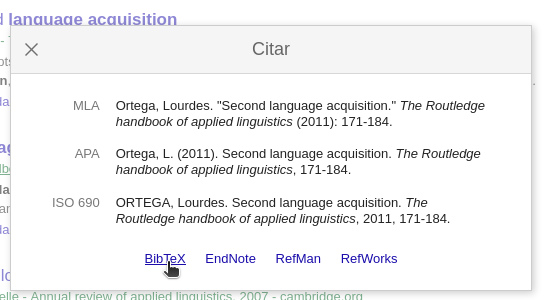
\includegraphics[width=0.50\textwidth]{bibtex.png}
    \caption{\textbf{\textit{Exemplo de onde clicámos para aceder ao texto pretendido}} \label{fig:imagem}}
\end{figure}

\newpage
Após isto é nos dado um texto semelhante ao seguinte

\begin{figure}[hbt]
    \centering
    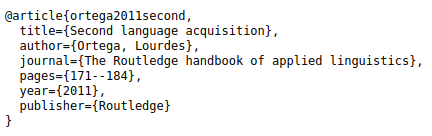
\includegraphics[width=0.50\textwidth]{textobib.png}
    \caption{\textbf{\textit{Texto pretendido}} \label{fig:imagem}}
\end{figure}

\section{Como usamos o ficheiro .bib para fazer as nossas referências bibliogŕaficas}
\Large

Para aplicarmos o ficheiro .bib para a apresentação das referências bibliográficas usámos as seguintes linhas:

Antes do início do documento:

\begin{figure}[hbt]
    \centering
    
\includegraphics[width=0.50\textwidth]{a.png}
    \caption{\textbf{\textit{Aplicação do ficheiro . bib}} \label{fig:imagem}}
\end{figure}

Onde queremos apresentar as referências:
\begin{figure}[hbt]
    \centering
    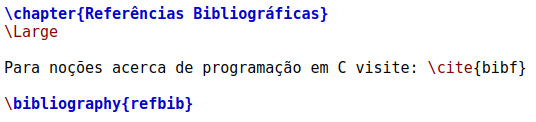
\includegraphics[width=0.50\textwidth]{c.png}
    \caption{\textbf{\textit{Aplicação do ficheiro . bib}} \label{fig:imagem}}
\end{figure}

\uline{NOTA}: As linhas acima apresentadas, não funcionaram da maneira esperada, tentámos várias outras formas e não conseguimos chegar ao resultado esperado. Mesmo assim achamos pertinente apresentar no relatório a nossa tentativa.

\newpage
\chapter{Conclusão} 
\label{cap:conclusao} % uma referência para o capítulo Conclusão
%\section{Conclusão}
\Large

O projeto prático de Laboratórios de Informática foi fundamental, tanto para a nossa aprendizagem acerca de conceitos sobre a disciplina como no âmbito da colaboração. A realização das diferentes etapas foi de extrema relevância, devido ao facto abordarmos aspetos cruciais no desenvolvimento das diferentes etapas necessárias para a construção de um projeto com qualidade.

Inicialmente com o desenvolvimento do programa com o código necessário para a resolução dos problemas apresentados nos diversos tópicos do trabalho final prático da unidade curricular Programação Imperativa, tivemos de adaptar o código para que pudesse ser possibilitada a entrada de argumentos e de opções no programa, permitindo o uso de diferentes ficheiros como entrada. Conseguimos perceber a grande vantagem dessa ferramenta no código. Com a estrutura de código que possibilita a entrada de ficheiros como argumentos no programa é possibilitada a implementação de diferentes ficheiros no programa pudendo mudar os dados facilmente. Sentimos algumas dificuldades nesta fase do trabalho, dificuldade sentida maioritariamente devido à elaboração de um algoritmo que cumprisse as condições necessárias para a implementação no programa dos ficheiros em forma de argumentos de forma correta. Considerámos ter sido a parte do trabalho que mais nos causou confusão. O uso de máquina virtual para a elaboração do projeto causou-nos alguma confusão muitas vezes para fazer as comunicações entre as nossas máquinas. Apesar disso considerámos que o uso das mesma acabou por nos trazer vantagens no desenvolvimento da nossa aprendizagem durante a realização do trabalho, foi aprendemos a trabalhar no sistema operativo Linux, percebendo algumas diferenças comparando com o sistema operativo Windows, presente nas máquinas de todos os envolvidos no trabalho. Considerámos a elaboração do presente trabalho também destacável no que toca a aprendizagem de funcionamento de novas plataformas. Com este trabalho percebemos a importância, para um bom projeto, da elaboração da documentação do código. Percebemos a pertinência do uso do “Doxygen”, considerando esta uma ferramenta muito facilitadora e prática, que, cumprindo os objetivos de uma boa documentação, facilita tanto a perceção do código, como na localização de certas partes do mesmo. Para o domínio necessário do “Doxygen” para a realização do presente trabalho, foi nos exigido apenas alguma pesquisa, pelo que considerámos a aplicação do mesmo relativamente simples. O uso de “LaTex”, foi para nós interessante, pois através disso percebemos como fazer relatório de um código de uma forma um pouco mais automatizada, percebendo até que esta plataforma acaba por ser um grande facilitador de trabalho, evitando a necessidade de fazer um relatório de forma manual, em certas situações. Consolidámos também o conceito de “MakeFile”, abordado pelo o professor durante o percurso letivo, percebendo como desenvolver e estruturar um ficheiro deste tipo funcional. Considerámos que a utilização de “Git” e “GitHub” no projeto, foi indispensável pois, considerámos esta ferramenta extremamente prática de se usar e excelente para a elaboração de projetos em grupo. Além disso percebemos a relevância desta ferramenta como uma plataforma de divulgação de projetos, podendo se revelar útil no futuro, como complemento de currículo. Percebemos também que esta pode ser uma plataforma útil para evitar perdas de trabalhos, pela possibilidade de ter em backups os mesmos na plataforma.

Em resumo, este projeto não foi apenas um exercício académico, mas sim uma forma de percebermos a grande diversidade de itens que podem ser usados no desenvolvimento de um projeto. Considerámos que este trabalho não só nos equipou com conhecimentos técnicos, mas

também com habilidades interpessoais e uma mentalidade pronta para enfrentar os desafios em constante evolução na área de redes de computadores.

\chapter{Referências Bibliográficas}
\Large

Para noções acerca de programação em C visite: \cite{bibf}

\bibliography{refbib}


\end{document}
